\chapter{Spettrometria di massa}

La spettrometria di massa è una tecnica analitica che misura la massa di
una molecola dopo averla ionizzata, ovvero dopo averle impartito una
carica elettrica.

La spettrometria di massa è in grado di fornire il peso molecolare, la
forma molecolare e anche delle informazioni strutturali attraverso la
frammentazione.

Esiste anche un'altra tecnica, ovvero l'analisi elementare o
microanalisi elementare, che può essere utilizzata per determinare la
formula minima. La formula minima non è quella molecolare.

La spettrometria di massa è una tecnica distruttiva, che però richiede
una quantità minima di campione; in molti casi bastano 10 \mu L di una
soluzione 10-6 M del campione.

La spettrometria di massa non è una tecnica spettroscopica, in quanto
non riguarda le interazioni della molecola con la luce.

Lo strumento utilizzato è lo spettrometro di massa. Questo strumento ha
tre parti principali, che si vedono nella figura \ref{fig:SpettrMS}.

\fullpicture{2_001}{Spettrometro di massa}{fig:SpettrMS}

Si hanno quindi tre parti principali
\begin{itemize}
  \item \textit{sorgente}: che converte le molecole neutre in ioni
  \item \textit{analizzatore}: che separa gli ioni prodotti dalla sorgente, a seconda del rapporto carica/massa.
  \item \textit{rivelatore}: che rivela gli ioni formati.
  \end{itemize}

A queste tre parti vanno aggiunti un sistema di introduzione del
campione e un sistema di elaborazione dei dati, che fornisce uno spettro
di massa, ovvero un grafico facilmente interpretabile.

Ora si vedono nel dettaglio la sorgente e l'analizzatore

\section{Sorgente}

La sorgente è la parte dello strumento dove si impartisce una carica
all'analita. È estremamente importante, in quanto il metodo di
ionizzazione utilizzato determina il numero di frammenti, la loro natura
e la loro abbondanza.

Esistono cinque metodi principali di ionizzazione: 
\begin{itemize}
  \item Impatto elettronico (EI)
  \item Ionizzazione chimica (CI)
  \item Ionizzazione per elettronebulizzazione o elettrospray (ESI)
  \item Bombardamento con atomi veloci (FAB)
  \item Ionizzazione laser assistita da matrice (MALDI)
\end{itemize}

Di queste tecniche, noi approfondiremo solo le prime tre.

In questi metodi di ionizzazione, si usa una certa quantità di energia
per ionizzare la molecola. Se l'energia coinvolta è molto alta, si parla
di una tecnica ``hard'', o molto aggressiva. In queste tecniche,
l'energia è così alta che la molecola ionizzata decompone in diversi
frammenti.

\begin{figure}[H]
  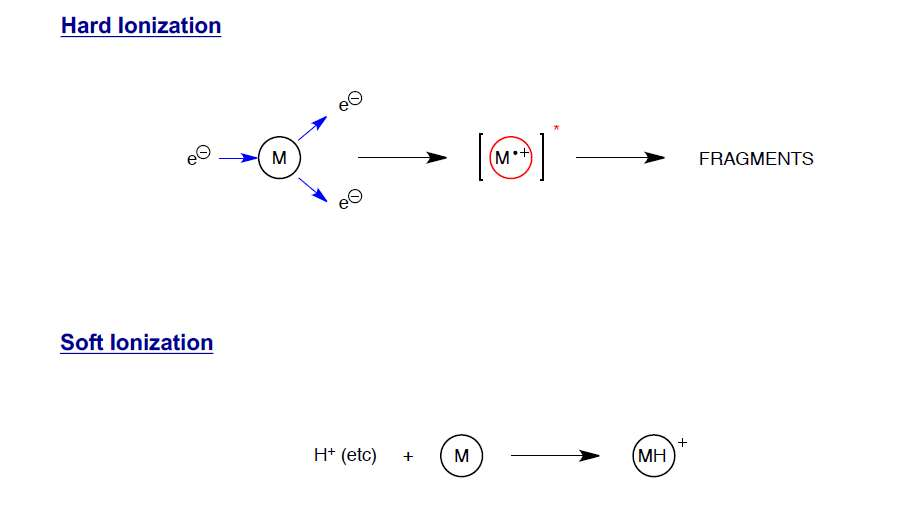
\includegraphics[width=0.7\textwidth]{2_002}
\end{figure}

I frammenti danno informazione strutturale, però si perde l'informazione
del peso molecolare.

Dall'altra parte, ci sono le tecniche a bassa energia, o tecniche
``soft''. Queste tecniche permettono di osservare la molecola integra
ionizzata (o ione molecolare).

Nella tabella sono elencate le cinque tecniche elencate prima, dalla più
hard, alla più soft.

L'impatto elettronico e la ionizzazione chimica sono le due tecniche più
hard e sono limitate allo studio di molecole relativamente piccole,
volatili e termicamente stabili.

Le altre tre tecniche sono tutte tecniche soft che permettono di
osservare la molecola integra ionizzata. Queste tecniche possono essere
utilizzate per studiare molecole grandi (fino a 6000 Da nel caso del FAB
e ESI, mentre nel caso del MALDI, fino a 500\,000 Da). Le molecole
analizzate possono essere non volatili e anche termolabili.

\paragraph{Impatto elettronico}

L'impatto elettronico è un metodo molto diffuso; in questo metodo, il
campione in fase gassosa viene bombardato da un fascio di elettroni ad
alta energia (normalmente 70 eV). L'impatto di un elettrone con la
molecola causa l'espulsione di un secondo elettrone dalla molecola,
generando un catione radicale, detto ione molecolare.

\marginpicture*{2_003}{Impatto elettronico}

\begin{center}
  \ce{M + e- -> M^{+.} + 2 e-}
\end{center}

Dallo ione molecolare è possibile ottenere il peso molecolare della
molecola incognita.

Tuttavia, in quanto l'energia utilizzata è molto alta, l'energia in
eccesso causa la decomposizione dello ione molecolare, che si spezza in
una serie di frammenti.

I frammenti danno informazione strutturale, poiché la frammentazione è
unica per ogni molecola. Questo è un vantaggio; lo svantaggio però è che
lo ione molecolare è difficile da osservare, quindi può essere
impossibile valutare il peso molecolare.

È possibile impiegare fasci con energia diversa. Questo porta a spettri
di massa diversi per la stessa molecola, in quanto a seconda
dell'energia, l'abbondanza dello ione molecolare e dei frammenti sarà
diversa.

Infatti, in figura \ref{fig:EnEI} si vede che man mano si diminuisce l'energia del
fascio elettronico, aumenta l'abbondanza dello ione molecolare, perché
la molecola si frammenta meno.

\fullpicture{2_004}{Effetto dell'energia dell'impatto elettronico sulla frammentazione}{fig:EnEI}

\paragraph{Ionizzazione chimica}

L'impatto elettronico in molti casi non permette di determinare il peso
molecolare; si utilizzano altre tecniche, come la ionizzazione chimica.

Si tratta di una tecnica meno aggressiva, che si basa sull'interazione
del campione vaporizzato con un reagente vaporizzato, di solito un acido
di Bronsted in fase gas.

Il reagente cede un protone all'analita per formare un adotto
molecola-protone, con massa M+1.

Il gas reagente deve essere in grado di formare un acido di Bronsted
molto forte; si utilizza metano o ammoniaca. Questo gas è presente nella
sorgente in grande eccesso rispetto all'analita, in modo tale che il
fascio elettronico ionizzi prevalentemente il gas reagente.

Nel caso del metano, la ionizzazione porta alla formazione del radicale
\ce{CH4^{+.}}. Questo reagisce con una seconda molecola di metano e, per
trasferimento di un protone, forma lo ione metanio \ce{CH5+}, che è un
acido di Bronsted estremamente forte.

Questo acido reagisce con l'analita, con una seconda reazione di
trasferimento di protone, per formare un adotto molecola-protone, con
carica positiva.

\paragraph{Elettrospray}

L'ultimo metodo di ionizzazione che vediamo è l'elettrospray (ESI).
L'elettrospray è una tecnica di ionizzazione soft, che consente di
analizzare molecole grandi e non volatili. Genera degli adotti della
molecola con un protone, del tipo M+1.

\halfpicture*{2_005}{Elettrospray}

In questo caso, il campione è sciolto in un solvente opportuno, in
presenza di piccole quantità di acido.

Il campione viene fatto passare attraverso un capillare, dove è stato
applicato un potenziale. A causa del potenziale, la soluzione viene
nebulizzata in piccole goccioline cariche, che desolvatandosi, esplodono
in gocce sempre più piccole.

Alla fine restano i soli ioni, che passano all'analizzatore. In questa
tecnica, si osservano quindi adotti M+1 con carica +1, però a seconda
dei siti di protonazione della molecola, è possibile la formazione di
adotti multicarica.

\subsection{Analizzatore}

L'analizzatore separa gli ioni in base al rapporto massa/carica. Il tipo
di analizzatore determina la risoluzione dello spettrometro di massa.

Ci sono diversi tipi di analizzatore:
\begin{itemize}
  \item a selettore magnetico
  \item a quadrupolo
  \item trappola ionica
  \item tempo di volo
  \item doppia focalizzazione
\end{itemize}

Noi vedremo solo i primi due analizzatori.

Il primo è molto diffuso, in quanto ha un'alta risoluzione e permette di
determinare la massa esatta.

Il secondo ha una risoluzione più bassa, però è molto economico e poco
ingombrante e anche molto utilizzato.

\paragraph{Analizzatore a tubo magnetico}

L'analizzatore a tubo magnetico è formato da un tubo lungo circa 1
metro, che è piegato con un raggio di curvatura \(r'\) ed è immerso in
un campo magnetico di intensità \(B\).

Per effetto del campo magnetico, gli ioni che entrano nel tubo subiscono
una deviazione dalla loro traiettoria rettilinea, che viene curvata.

\fullpicture*{2_006}{Analizzatore a tubo magnetico}

La nuova traiettoria curvilinea ha un raggio di curvatura \(r\), che
dipende dalla massa dello ione. Quindi, per determinati valori di
potenziale del campo magnetico, esiste solo un valore di massa/carica,
per cui il raggio della traiettoria curvilinea dello ione coincide con
il raggio di curvatura del tubo.

Quindi solo questi ioni sono in grado di arrivare al rivelatore. Se poi
si varia il valore del campo magnetico, si possono far uscire ioni con
rapporto massa/carica differente, a tempi diversi.

\paragraph{Analizzatore a quadrupolo}

L'analizzatore a quadrupolo è costituito da quattro barre metalliche, al
quale viene applicato una differenza di potenziale, generata da una
corrente continua e da una corrente alternata. in questo modo, quando le
due barre verticali hanno un potenziale negativo, le altre due barre
hanno potenziale positivo, e viceversa.

Gli ioni che entrano nel tunnel delimitato dalle barre, assumono una
traiettoria a zig-zag, la cui oscillazione dipende, oltre dal potenziale
applicato, ma anche dal rapporto massa/carica dello ione.

\fullpicture*{2_007}{Analizzatore a quadrupolo}

In questo modo, ad un determinato valore di potenziale, soltanto ioni
con uno specifico rapporto massa/carica riusciranno ad avere una
traiettoria stabile e potranno uscire per andare al rivelatore

Variando poi il potenziale, sarà possibile far uscire gli ioni con
diverso rapporto massa/carica a tempi diversi.

Come già detto, questo tipo di analizzatore è più economico e meno
ingombrante, però presenta diversi svantaggi: - bassa risoluzione - il
limite superiore per il rapporto massa/carica che è piuttosto basso (non
superiore a 2500 Da).

Infine, non può essere accoppiato a sorgenti MALDI

\section{Spettro di massa}

Lo spettro di massa è simile a quello in figura. Nell'asse orizzontale
si trova $\nicefrac{m}{z}$, mentre nell'asse verticale, si trova l'abbondanza
relativa.

Ognuna delle barre è uno ione con un determinato rapporto massa/carica.
L'altezza indica l'abbondanza dello ione.

L'abbondanza è normalizzata in base al picco più abbondante, che si
chiama picco base, a cui viene assegnata un'abbondanza 100. L'abbondanza
degli altri picchi è data in base al picco base.

Nello spettro di massa va anche indicato il tipo di ionizzazione; una
ionizzazione più spinta produrrà uno spettro con più picchi, mentre una
ionizzazione soft produrrà uno spettro con pochi picchi.

Nello spettro in figura, lo spettro è stato ottenuto da una sorgente a
impatto elettronico, quindi è presente una grande frammentazione.

\fullpicture*{2_008}{Spettro di massa}

Nello spettro si vede lo ione molecolare, però si vedono molti picchi
con un rapporto $\nicefrac{m}{z}$ più basso.

Nello spettro si vede anche che tutti i rapporti massa/carica sono
arrotondati all'unità. Questo significa che lo spettro è a bassa
risoluzione. Se invece si fa uno spettro ad alta risoluzione, il
rapporto $\nicefrac{m}{z}$ è arrotondato alla quarta cifra decimale.

Si nota anche che attorno allo ione molecolare sono presenti dei picchi
più piccoli, con massa M+1 e M+2 e sono chiamati picchi isotopici.
Derivano dai diversi isotopi presenti nella molecola.

\paragraph{Ione molecolare}

Lo ione molecolare corrisponde alla molecola ionizzata integra, ovvero
senza frammentazioni. La sua massa coincide con il suo peso molecolare.
L'intensità dello ione molecolare dipende dal metodo di ionizzazione.

Per lo ione molecolare vale la regola dell'azoto, ovvero lo ione
molecolare ha massa pari, a meno che la molecola non contenga un numero
dispari di atomi di azoto. Questa è una regola importante per
determinare il peso molecolare della molecola.

La regola vale soltanto per molecole contenenti C, H, O, S, X, N.

Nell'impatto elettronico, si formano solo ioni monocarica, pertanto i
valori $\nicefrac{m}{z}$ coincidono con la massa dello ione. Normalmente si osservano
cationi o cationi radicali.

\paragraph{Picchi isotopici}

La maggior parte dei composti organici, sono composti da C, H, O, N;
tutti questi elementi hanno degli isotopi naturali, che hanno masse
diverse.

La spettrometria di massa è in grado di separare gli ioni con isotopi
differenti, in quanto gli isotopi hanno massa diversa.

\fullpicture*{2_009}{Picchi isotopici}

Si prenda come esempio lo spettro del metano. In questa molecola è
presente solo un atomo di carbonio. Il carbonio si trova in natura in
due isotopi \ce{^{12}C} e \ce{^{13}C}; quest'ultimo ha un'abbondanza bassa (circa
l'1\%). Quindi ogni 100 molecole di metano, si avrà una molecola di
metano contenente \ce{^{13}C}, piuttosto che \ce{^{12}C}.

Quindi, la maggior parte delle molecole avrà una massa di 16 Da, mentre
la molecola con il \ce{^{13}C} avrà una massa di 17 Da.

La spettrometria di massa riesce a vedere entrambe le molecole. Infatti
si vede lo ione molecolare a 16, però si vede un picco con un abbondanza
di circa 1\%, che corrisponde alla molecola di metano con il 13C.

Questo succede anche per gli altri elementi componenti le molecole
organiche.

\begin{table}
\begin{tabular}{ccc}
Elemento & Isotopi & Massa esatta\\
H & \ce{^{1}H} (100 \%) & 1.00783\\
& \ce{^{2}H} (0.016 \%) & 2.01410\\
C & \ce{^{12}C} (100 \%) & 12.000\\
& \ce{^{13}C} (1.08 \%) & 13.0034\\
N & \ce{^{14}N} (100 \%) & 14.0031\\
& \ce{^{15}N} (0.38 \%) & 15.0001\\
O & \ce{^{16}O} (100 \%) & 15.9949\\
& \ce{^{17}O} (0.04 \%) & 16.9991\\
& \ce{^{18}O} (0.2 \%) & 17.9992\\
\end{tabular}
\caption{Abbondanza isotopica}
\label{tab:IsoLeggeri}
\end{table}

Come si nota nella tabella \ref{tab:IsoLeggeri}, l'isotopo più
abbondante è quello più leggero. Però ci sono delle eccezioni a questa
regola. Le eccezioni più importanti sono il cloro e il bromo.

\fullpicture*{2_010}{Spettro dell'acido cloridrico}

Nel caso del cloro, ci sono due isotopi, uno più leggero \ce{^{35}Cl} e uno più
abbondante \ce{^{37}Cl}. L'isotopo più pesante ha un'abbondanza relativa di
circa il 33 \%, per cui non è trascurabile. Questo significa che il
picco isotopico a M+2 sarà abbastanza grande, in particolare, tra i due
picchi isotopici si troverà una relazione di 3:1.

Nel caso del bromo, questa caratteristica è ancora più importante, in
quanto il \ce{^{79}Br} ha un'abbondanza relativa del 100\%, però il \ce{^{81}Br} ha
un'abbondanza di 98 \%. Questo significa che nello spettro di massa di
una molecola che contiene bromo, si vedranno due picchi isotopici a M e
M+2, con un rapporto di intensità di 1:1.

\fullpicture*{2_011}{Picchi idotopici per il cloro}

I picchi isotopici rendono molto agevole la determinazione della
presenza del cloro o del bromo nella molecola.

Un altra cosa importante da ricordare è che la spettrometria di massa è
che si vede la somma della massa degli isotopi e non la somma dei pesi
atomici.

\fullpicture*{2_012}{Picchi isotopici per il bromo}

Questo comporta che non si può determinare lo spettro a partire dal peso
molecolare, in quanto il peso molecolare è la media pesata della massa
degli isotopi.

Quindi si distinguono il peso molecolare, la massa nominale e la massa
esatta.
\begin{itemize}
  \item Peso Molecolare: somma delle masse atomiche degli elementi che
  costituiscono la molecola. La massa atomica è una media pesata delle
  masse dei diversi isotopi di un determinato elemento. Il peso molecolare
  non viene visto allo spettrometsro di massa.
  \item Massa nominale: somma
  delle masse degli isotopi più abbondanti degli elementi che
  costituiscono la molecola, arrotondati all'unità
  \item Massa esatta: somma
  delle masse degli isotopi più abbondanti senza che questi valori vengano
  approssimati. La massa esatta è quella che si misura allo spettrometro
  di massa
\end{itemize}

Quando aumenta la complessità della molecola, quindi il numero di atomi,
è più difficile calcolare l'abbondanza dei picchi isotopici.

Ad esempio, nello spettro a bassa risoluzione del benzene, si vede il
picco dello ione molecolare a 78.

Per questa molecola, l'unica specie che contribuisce allo ione
molecolare è il \ce{^{12}C6^{1}H6}, ovvero tutti gli atomi di carbonio
sono 12C e tutti gli atomi di idrogeno sono \ce{^{1}H}.

Quando si va a vedere il picco isotopico a M+1, ci sono più specie che
possono contribuire, come ad esempio 12C5 13C 1H6, oppure 12C6 1H5 2H,
dove rispettivamente sono stati sostituiti un atomo di carbonio con il
suo isotopo e un atomo di idrogeno con il suo isotopo.

\fullpicture*{2_013}{Spettro del 2-cloropropano}

Guardando invece lo spettro del 2-cloropropano, si vede che nello
spettro di massa è presente un picco isotopico con intensità relativa
1:3 rispetto a quella del picco dello ione molecolare.

Se invece si prende una molecola contenente un atomo di bromo, come
1-bromopropano, si trovano due picchi isotopici con una abbondanza
relativa di 1:1.

Se si aumenta il numero di atomi di cloro o di bromo, si vede che, a
seconda del numero di atomi aggiunti, si ha una distribuzione isotopica
specifica.

\fullpicture*{2_014}{Spettro del 1-bromopropano}

Questi dati sono già tabulati sottoforma di grafici, per cui, se si vede
una distribuzione isotopica strana, si va a vedere la tabella e si
riconosce la presenza di più atomi per comparazione.

\marginpicture*{2_015}{Distribuzione dei picchi isotopici}

Quindi si vede che la distribuzione dei picchi isotopici è specifica
della molecola, quindi utilizzando l'intensità di questi picchi. È
possibile determinare la formula molecolare.

È importante anche il processo inverso, ovvero calcolare la
distribuzione di intensità dei picchi isotopici a partire da una forma
molecolare.

Esistono delle formule, però non vengono più utilizzate, in quanto,
oggigiorno, si utilizzano dei programmi come ChemDraw che consentono di
determinare la distribuzione isotopica che si vede alla massa.

\subsubsection{Formula molecolare}

Per determinare la formula molecolare si possono utilizzare tre metodi:
\begin{itemize}
  \item Si può utilizzare una combinazione tra la spettrometria di massa, che
  dà il peso molecolare, e l'analisi elementare, che fornisce la formula
  minima
  \item Si può utilizzare l'abbondanza relativa dei picchi isotopici
  \item Si può utilizzare anche la massa esatta
\end{itemize}

\paragraph{Analisi elementare}

L'analisi elementare è un metodo chimico, nel quale si analizzano i gas
prodotti dalla combustione del campione con \ce{O2}. L'analisi elementare
necessita di conoscere la massa del campione.

Il campione viene bruciato in corrente di ossigeno. I prodotti di
combustione sono acqua e ossidi di carbonio, azoto e zolfo, se presenti
nella molecola. La quantità dei prodotti di combustione viene
determinata.

In seguito, sapendo che gli atomi di carbonio producono altrettante
molecole di \ce{CO2}, si può determinare il numero di carboni nella
molecola.

Inoltre, sapendo che l'acqua contiene due atomi di idrogeno, è possibile
trovare il numero degli atomi di idrogeno della molecola, pari alla metà
delle molecole d'acqua.

Si può determinare direttamente la quantità di carbonio, idrogeno, azoto
e zolfo.

L'ossigeno non è direttamente determinabile con l'analisi elementare, in
quanto l'ossigeno presente negli ossidi proviene sia dagli atomi di
ossigeno presenti nella molecola, sia dagli atomi di ossigeno del
flusso. La quantità di ossigeno deve essere calcolata in modo indiretto.

Ad esempio, dall'analisi elementare risulta che la composizione in
grammi di un campione è di:

\begin{center}
  C, 53.04; H, 3.89; N, 7.73
\end{center}

Il composto in questione contiene, oltre a questi tre elementi, anche
l'ossigeno.

Facendo la somma dei grammi, si nota che non raggiunge il 100. Quindi si
vede che il rimanente è composto da elementi che l'analisi elementare
non riesce a determinare in modo diretto.

Dal problema, si vede che l'unico elemento rimanente è l'ossigeno, che
quindi può essere calcolato indirettamente. L'ossigeno è presente con
una massa di 35.33 grammi.

Dalle quantità in grammi, attraverso la massa molare, si passa al numero
di moli presenti nel campione.

Prendendo il numero di moli più piccolo, si vanno a trovare i rapporti
molari all'interno della molecola, ottenendo così la formula minima.
Quindi, nel caso precedente, la formula bruta è \ce{C8H7NO4}.

Per determinare la formula molecolare, bisogna avere il rapporto tra la
formula molecolare ottenuta con la spettrometria di massa e la massa
della formula minima.

Ad esempio, la massa molecolare ottenuta per questa molecola è di 181.
Se si ottiene un rapporto $\nicefrac{m}{z}$ pari a 181, allora la formula minima
coincide con la formula molecolare.

\paragraph{Picchi isotopici}

Il secondo metodo per determinare la formula molecolare è il metodo dei
picchi isotopici, che viene utilizzato se si ha a disposizione solo uno
spettro a bassa risoluzione.

La capacita di uno spettrometro di massa di difefrenziare le masse
è generalemente espressa dalla risoluzione, che è definita come:
\[
  R = \frac{m}{\Delta m}
\]

Il problema degli spettri a bassa risoluzione è che per lo stesso
rapporto massa/carica, sono possibili diverse formule molecolari.
Tuttavia, la distribuzione dei picchi isotopici è unica anche se la
risoluzione è bassa.

Quindi si compara l'intensità dei picchi isotopici con i dati tabulati,
che sono contenuti nelle tabelle di Beyron.

Queste tabelle contengono solo i dati per le molecole organiche
contenenti sono carbonio, idrogeno, ossigeno e azoto.

Questo metodo perde efficacia per pesi molecolari maggiori di 250 Da.

\paragraph{Massa esatta}

L'ultimo metodo che si va a vedere è la determinazione della formula
molecolare mediante la massa esatta. In questo caso, si dispone di uno
spettro ad alta risoluzione, quindi il rapporto massa/carica è
arrotondato alla quarta cifra decimale.

Per un valore di massa esatta è quindi possibile una sola formula
molecolare. Quindi, dopo aver registrato lo spettro, si va a trovare in
una tabella a quale formula molecolare corrisponde la massa esatta.

Le tabelle contengono sono formule molecolari contenenti solo carbonio,
idrogeno, ossigeno e azoto.

Se la molecola contiene altri elementi, allora si utilizzano le
calcolatrici online, che sono più complete.

\section{Frammentazioni}

Se si è in grado di interpretare i picchi di frammentazione dello
spettro, allora si possono ricavare delle informazioni strutturali.

Prima di andare a studiare i diversi tipi di frammentazione, bisogna
capire che cos'è lo ione molecolare.

Lo ione molecolare è un catione radicale ad alta energia; nel caso degli
alcani, l'elettrone è delocalizzato su tutta la molecola. Il miglior
modo per rappresentarlo è mettendo lo ione tra parentesi quadrate, con
il simbolo radicale.

Se si sta lavorando con una molecola insatura o con eteroatomi,
l'impatto elettronico va sicuramente in uno di questi atomi. Si può
considerare il catione radicale come localizzato sull'eteroatomo o
sull'instaurazione.

Si prendano esempio queste reazioni

\begin{figure}[H]
  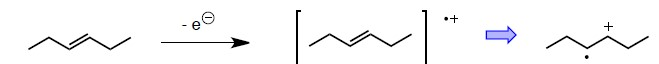
\includegraphics[width=\textwidth]{2_016}
\end{figure}

\begin{figure}[H]
  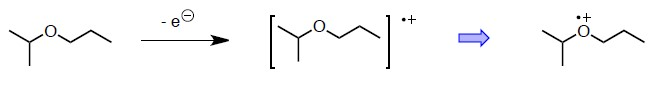
\includegraphics[width=\textwidth]{2_017}
\end{figure}

\begin{figure}[H]
  
\includegraphics[width=\textwidth]{2_018}
\end{figure}

Ad esempio, nell'etere, si ha un eteroatomo, l'ossigeno, che è parte del
corpo carbonioso. L'impatto elettronico va a rimuovere un elettrone di
non legame dell'ossigeno. Lo ione molecolare ottenuto può essere anche
rappresentato con il radicale localizzato nell'atomo di ossigeno.

Nel caso di un alchene, avviene più o meno la stessa cosa. L'impatto
elettronico va a creare uno ione molecolare con l'elettrone spaiato su
un carbonio del doppio legame e la carica positiva sull'altro.

L'ultimo esempio è un chetone, dove si ha sia l'integrazione che la
presenza di un eteroatomo. L'impatto elettronico strappa un elettrone
dall'eteroatomo, quindi la forma più importante è quella con il radicale
e la carica positiva localizzata nell'ossigeno.

\marginbox*{Si ricordi che la singola freccia indica lo spostamento di un solo
elettrone, mentre la doppia freccia indica lo spostamento di due
elettroni.}

Nelle frammentazioni, si ha anche lo spostamento di singoli elettroni.

\begin{figure}[H]
  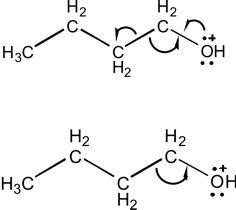
\includegraphics[width=0.3\textwidth]{2_019}
\end{figure}

Ad esempio, nella prima reazione si vede lo spostamento diretto del
radicale, mentre nella seconda reazione si vede lo spostamento di un
legame, ovvero due elettroni. Nella prima reazione avviene anche una
rottura omolitica di un legame, quindi i due elettroni vanno in parti
diverse della molecola. Nel secondo esempio, avviene una rottura
eterolitica.

\subsection{Tipi di frammentazioni}

Esistono due grandi classi di frammentazioni dello ione molecolare

\begin{itemize}
\item
  Frammentazioni semplici o scissioni: scissioni omolitiche o
  eterolitiche di un legame della molecola
\item
  Riarrangiamenti o trasposizioni: si rompono dei legami, ma si formano
  anche nuovi legami.
\end{itemize}

\subsubsection{Scissioni}

Nel caso di una rottura omolitica, i due elettroni del primo legame, si
separano e si muovono indipendentemente, per formare un radicale e un
catione.

\begin{figure}[H]
  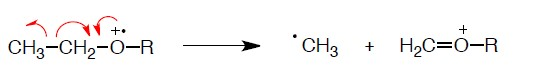
\includegraphics[width=0.8\textwidth]{2_020}
\end{figure}

Mentre nella rottura eterolitica, i due elettroni del legame che si
rompe migrano insieme. Se la rottura eterolitica avviene in un catione
radicalico, si forma un catione e un radicale. Se invece la rottura
avviene su un catione, allora i prodotti sono un catione e una molecola
neutra.

\begin{figure}[H]
  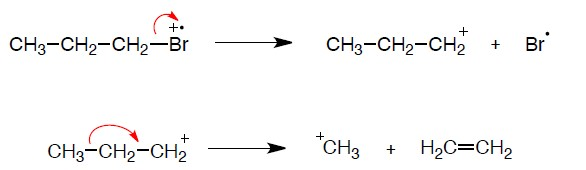
\includegraphics[width=0.8\textwidth]{2_021}
\end{figure}

Nel primo caso, il catione formato è un catione generico, quindi si può
assegnare un rapporto massa/carica. Il catione viene identificato come
M-15, in quanto avviene la perdita di un metile, che ha massa 15.

Nel secondo caso, il primo catione può essere identificato sia con il
rapporto massa/carica, sia utilizzando M-Br, che sta a indicare la
perdita di un atomo di bromo dalla molecola.

Lo stesso avviene anche nel secondo catione, che può essere identificato
tramite il suo rapporto massa/carica, ma anche tramite M-metile, in
quanto avviene la perdita di un metile.

Si nota anche che la rottura omolitica avviene solo se è presente un
catione radicale, mentre la rottura eterolitica può avvenire anche in
cationi. Questi cationi possono essere frammenti della molecola.

I frammenti ottenuti dalla frammentazione dello ione molecolare possono
a loro volta frammentare, per formare un catione e una molecola neutra.

\paragraph{Riarrangiamenti}

Per i riarrangiamenti, sono presenti due meccanismi diversi:
\begin{itemize}
  \item Riarrangiamento di McLafferty
  \item Retro Diels-Alder
\end{itemize}

Noi studieremo solo il riaggangiamento di McLafferty.
Il riarrangiamento di McLafferty è molto comune. Questa reazione ha
bisogno di due requisiti:
\begin{itemize}
  \item La molecola deve avere un gruppo funzionale
  in grado di formare un catione radicale localizzato
  \item La molecola deve
  avere almeno un atomo di idrogeno in posizione \(\gamma\) rispetto al
  gruppo funzionale.
\end{itemize}

\marginpicture*{2_022}{Requisiti per il riarrangiamento di McLafferty.
Questa è la struttura generale di una molecola in grado di dare il
riarrangiamento di McLafferty. L'atomo Z può essere carbonio, azoto o
ossigeno.}

I composti in grado di dare questo riarrangiamento sono gli
alcheni, le immine e i composti carbonilici. Per composti carbonilici si
intendono chetoni, aldeidi, esteri, ma anche acidi carbossilici.

\begin{figure}[hbtp]
  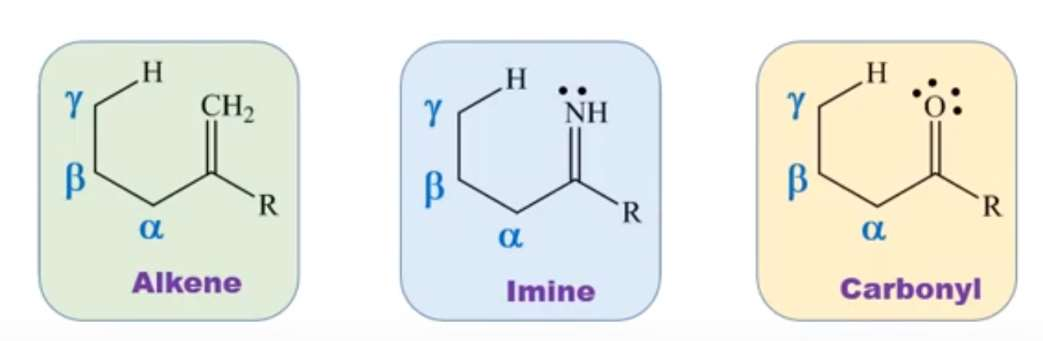
\includegraphics[width=0.6\textwidth]{2_023}
  \caption{Classi di molecole adatte per il riarrangiamento di McLafferty}
\end{figure} 

Il raggiungimento avviene tramite uno stato di transizione a sei
termini, nel quale tutti gli elettroni coinvolti nella frammentazione,
si muovono allo stesso tempo.

\begin{figure}[H]
  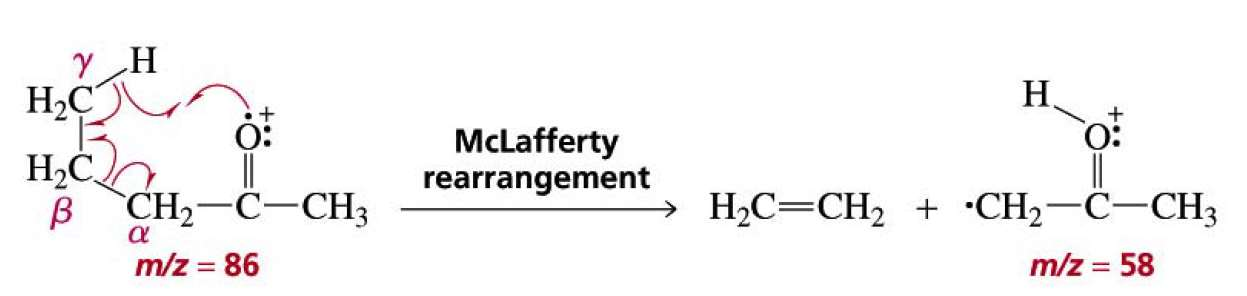
\includegraphics[width=0.8\textwidth]{2_024}
\end{figure}

Come si vede nella reazione, partendo da un aldeide, si vede che la
ionizzazione porta alla formazione di un catione radicalico localizzato
sull'ossigeno. Nello stato di transizione, si vede che gli elettroni si
muovono tutti allo stesso tempo.

\begin{figure}[H]
  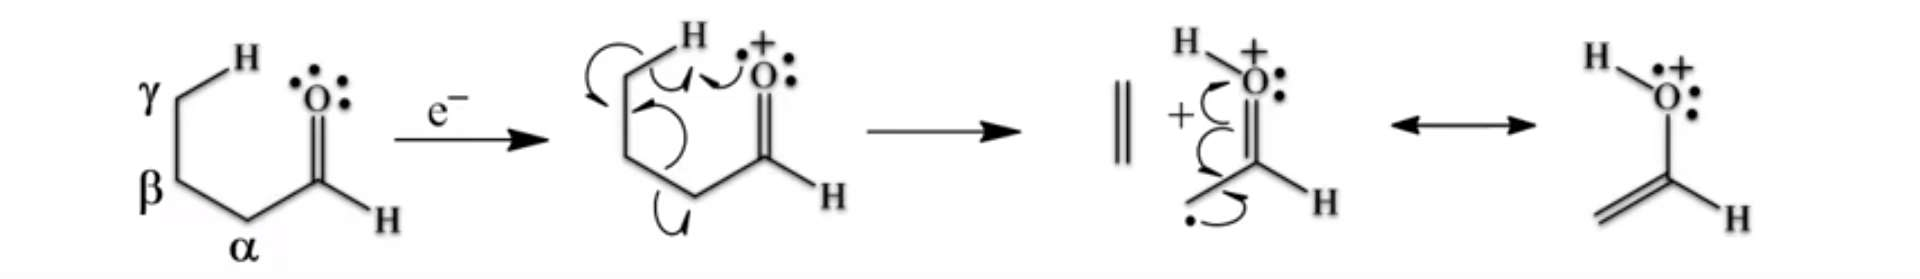
\includegraphics[width=0.9\textwidth]{2_025}
\end{figure}

Il radicale attacca l'idrogeno in \gamma{} formando un nuovo legame; si
rompe il legame C-H con scissione omolitica. La rottura del legame porta
alla formazione di un secondo legame tra i carboni in posizione \beta{}
e \gamma{}, e si rompe il legame tra i carboni \alpha{} e \beta{}.

Quindi si forma una molecola neutra e un catione radicalico; il catione
radicale, per risonanza, tautomerizza nella forma enolica.

Il riarrangiamento di McLafferty è rappresentato anche come movimento di
coppie di elettroni. In questo caso, si localizza il radicale
nell'eteroatomo, dopodiché, il doppio legame attacca l'idrogeno in
\gamma{}. Il legame dell'idrogeno si rompe e forma un doppio legame tra
il carbonio \beta{} e \gamma{}. Il legame tra il carbonio \alpha{} e
\beta{} si rompe e gli elettroni del legame si spostano tra il carbonio
carbonilico e il l'\alpha-carbonio.

\begin{figure}[H]
  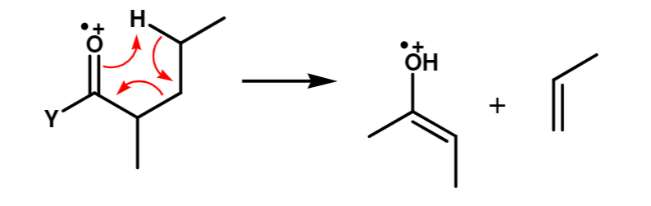
\includegraphics[width=0.7\textwidth]{2_026}
\end{figure}

Il risultato di questa reazione è direttamente la forma enolica

\subsection{Regole sulla frammentazione}

Quindi si possono ricavare una serie di regole per la frammentazione.
Una frammentazione dà luogo a solo un frammento con carica positiva.
Questo frammento è chiamato ione frammento ed è l'unico che dà un picco
nello spettro di massa, in quanto il rivelatore vede cationi o radicali
cationi.

Come esempio, si vede lo spettro della butirraldeide. La butiraldeide dà
luogo al riarrangiamento di McLafferty, formando un olefina neutra e un
catione radicalico.

\begin{figure}[H]
  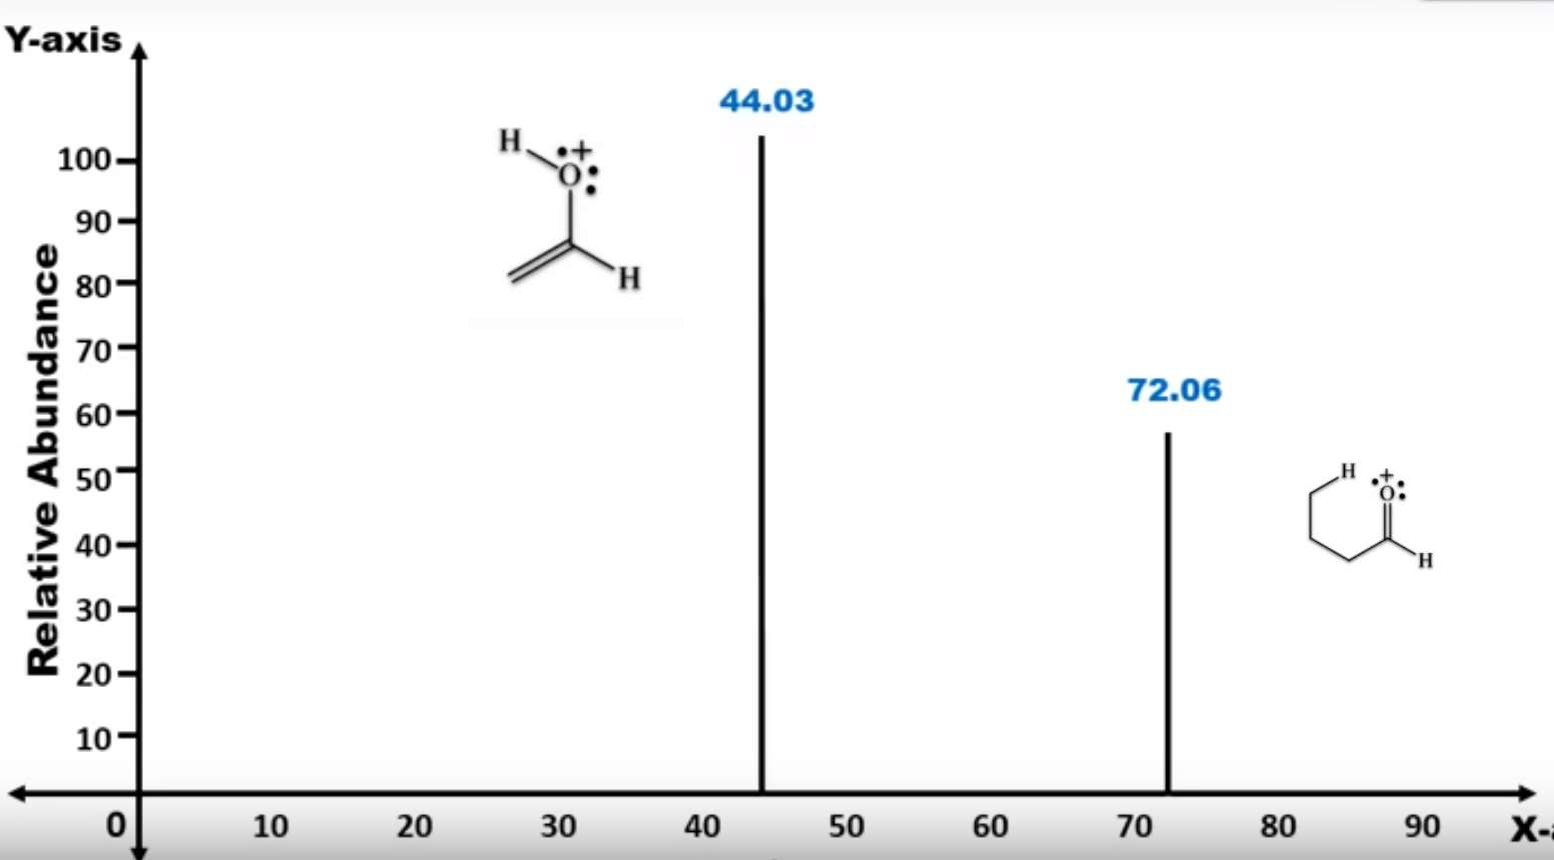
\includegraphics[width=\textwidth]{2_027}
\end{figure}

Nello spettro di massa si vede un picco a 72, che corrisponde allo ione
molecolare, mentre il picco a 44 corrisponde al catione radicale formato
nel riagganciamento di McLafferty.

Un altra regola è l'estensione della regola dell'azoto. La regola può
essere espressa come:

\begin{quoting}
Le molecole con un numero pari di atomi di azoto hanno lo ione
molecolare con una massa pari. I frammenti cationici hanno massa
dispari, mentre i frammenti cationici radicalici hanno massa pari

Viceversa, una molecola con un numero di atomi dispari ha lo ione
molecolare con massa dispari. I frammenti cationici hanno massa pari,
mentre i frammenti cationici radicalici hanno massa dispari.
\end{quoting}

\begin{figure}[H]
  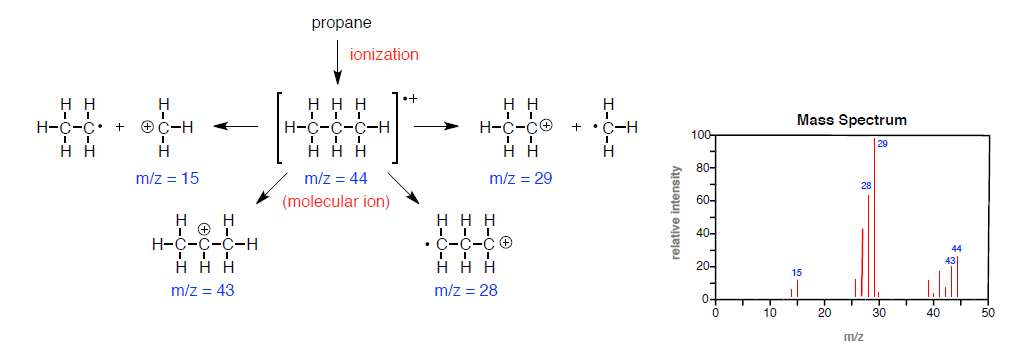
\includegraphics[width=\textwidth]{2_028}
\end{figure}

Questo è illustrato nell'esempio del propano. Il propano non presenta
atomi di azoto, quindi il suo numero di atomi è pari. La sua massa è 44.

La frammentazione del propano dà luogo a diversi frammenti. Tutti i
frammenti di tipo cationico hanno massa dispari, mentre i frammenti di
tipo cationico radicalico hanno una massa pari.

Gli ioni frammento possono a loro volta frammentare, per fornire una
molecola neutra e un catione.

I picchi devono seguire una logica. In genere, si riscontrano picchi a
M-1 e M-2, per perdita di idrogeno. Nonsi dovrebbero osservare frammenti
del tipo dall'intervallo M-3 a M-14, ne dall'intervallo M-23 a M-25.

In mezzo a questi due intervalli si trovano spesso frammenti con M-15
(perdita di un metile), M-19 (perdita del fluoro) e M-20 (perdita di
fluoro e di idrogeno).

Si trova spesso anche M-18, che rappresenta la perdita di acqua.

Un altra cosa osservata è che non tutte le molecole frammentano
facilmente. Ci sono molecole che frammentano molto più facilmente poiché
il loro ione molecolare è più attivo.

In generale, si osserva che alcoli, acidi carbossilici e alcani
ramificati sono i composti che tendono più a frammentare nella
spettrometria di massa. Quindi questi composti daranno molti frammenti,
e quindi lo ione molecolare è poco abbondante.

Al contrario, i composti aromatici, alcheni e alcani lineari non hanno
molta tendenza a frammentare, quindi l'abbondanza degli ioni frammenti è
bassa, mentre l'abbondanza dello ione molecolare è alta.

In principio, quando si ionizza una molecola, ogni legame può rompersi.
Però si vede che alcune frammentazioni sono più facili di altre e quindi
danno luogo a picchi più intensi nello spettro di massa.

Le frammentazioni favorite sono quelle dei legami più deboli e, in
secondo luogo, è favorita la frammentazione che dà luogo a frammenti
stabili. La stabilità è quella dei carbocationi, quindi il metile è meno
stabile e i più stabili sono i carbocationi stabilizzati per risonanza.

\begin{figure}[H]
  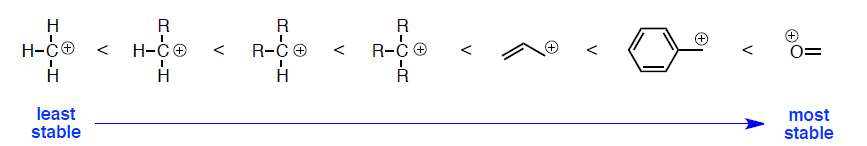
\includegraphics[width=\textwidth]{2_029}
\end{figure}

Questa regola porta alla conclusione che, in presenza di un alcano
ramificato, si favorisce la frammentazione dei legami vicini alla
ramificazione, poiché danno dei carbocationi che sono più sostituiti e
quindi più stabili.

È anche favorita la frammentazione del legame \alpha-\beta{} rispetto ad
un eteroatomo o ad un doppio legame, in quanto si formano dei
carbocationi stabilizzati per risonanza.

A parità di altre condizioni, il gruppo alchilico più grande tende a
staccarsi.

\begin{figure}[H]
  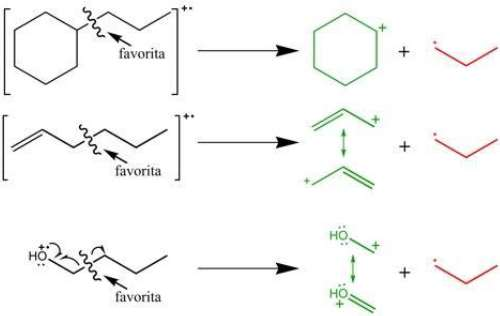
\includegraphics[width=0.8\textwidth]{2_030}
\end{figure}

Nel primo esempio, si ha un alcano ramificato ciclico, quindi è favorita
la perdita del ciclo, quindi la frammentazione del legame che lega la
catena al ciclo.

Nel secondo caso, è favorita la frammentazione del legame \alpha-\beta{}
rispetto all'instaurazione, poiché si forma un carbocatione che è
stabilizzato per risonanza.

Lo stesso accade nel caso di un alcol, dove è favorita la frammentazione
del legame \alpha-\beta{} rispetto all'alcol, in quanto il carbocatione
ottenuto è stabilizzato per risonanza

\section{Frammentazioni dei gruppi funzionali}

Si ricordi che il nostro obiettivo non è quello di spiegare ogni singolo
picco dello spettro di massa. Però bisogna essere in grado di predire le
frammentazioni principali di una molecola.

\fullpicture*{2_031}{Frammentazioni dei vari gruppi funzionali}

Inoltre bisogna anche essere in grado di identificare frammenti o
perdite diagnostiche dei gruppi funzionali.

\subsection{Alcani}

Negli alcani, lo ione molecolare è poco intenso, però è visibile. Tutti
i legami C-C dello ione molecolare possono frammentare, infatti si
vedono dei picchi separati da 14 $\nicefrac{m}{z}$, che corrispondono alla perdita di
metileni, dove l'intensità massima si ha per i frammenti con tre o
quattro atomi di carbonio.

Questi segnali corrispondono a frammenti con massa 43 e 57.

\begin{figure}[H]
  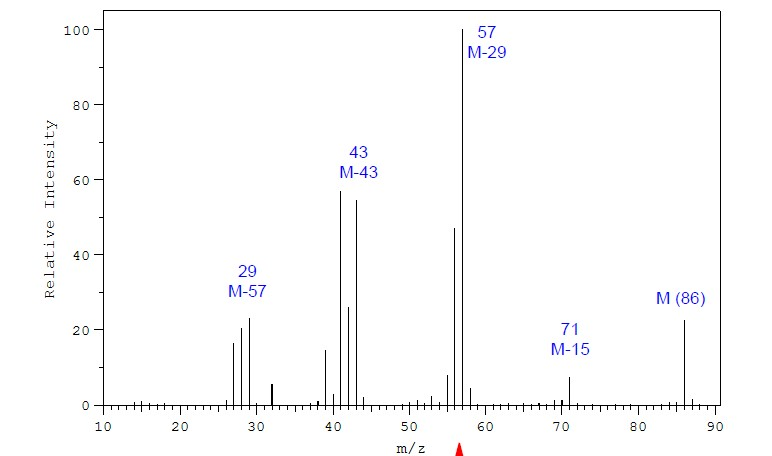
\includegraphics[width=\textwidth]{2_032}
  \caption{Spettro del n-esano}
\end{figure}

In figura, si vede lo spettro dell'esano. In questo spettro si vede lo
ione molecolare, con massa 86, che è pari perché non c'è nessun azoto.

Il picco base corrisponde a 57, che è dispari e quindi è un catione.
Questo picco corrisponde ad un composto a quattro atomi di carbonio
Inoltre si vede la serie di picchi 71-57-43-29, che sono separati da 14
unità di massa. Lo stesso andamento si avrà per alcani più lunghi.

\fullpicture*{2_033}{Spettro del n-pentadecano}

\begin{figure}[H]
  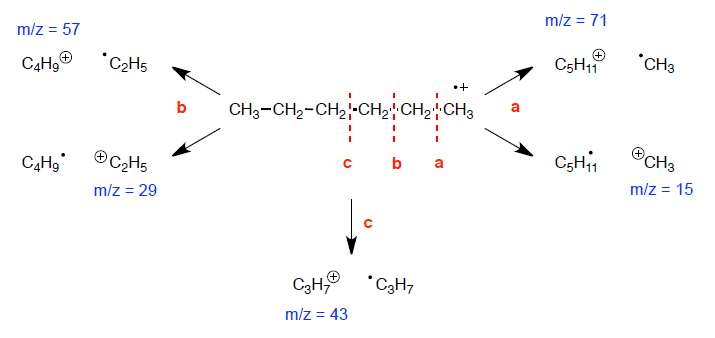
\includegraphics[width=\textwidth]{2_034}
\end{figure}

In questa figura si vede la frammentazione dell'esano. Nello ione
molecolare dell'esano, si hanno tre legami C-C che possono frammentare.

Se si frammenta il legame a, si può lasciare la carica positiva sul
frammento più grande o su quello più piccolo. Quindi questa
frammentazione potrebbe dare un frammento con $\nicefrac{m}{z}$ uguale a 71 oppure
uguale a 15 (metile).

Questo succede anche se si frammenta il legame b. La rottura può
lasciare la carica positiva sul frammento più grande, che darà un picco
a 57, o sul frammento più piccolo, che darà un picco a 29.

Se invece si frammenta il legame c, è possibile solo la formazione di un
carbocatione con tre carboni, quindi con massa 43.

La figura vista prima è un vero e proprio schema di reazione, con
reagenti e prodotti. Però esiste un secondo modo per rappresentare la
frammentazione, che è rappresentato nella figura sottostante.

\begin{figure}[H]
  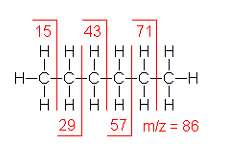
\includegraphics[width=0.4\textwidth]{2_035}
\end{figure}

Prendendo la molecola, si indica la frammentazione con una linea
verticale e, con una linea orizzontale, si indica dove si lascia la
carica positiva. Il numero rappresenta la massa del frammento.

Si vedono anche degli spettri di alcani a catena lunga. Si ha sempre una
separazione tra i picchi di 14 unità. I picchi più intensi sono quelli a
43 e 57; in seguito, l'abbondanza cala velocemente.

Negli alcani ramificati, si vede che il profilo degli alcani lineari
presenta una discontinuità.

\fullpicture*{2_036}{Spettro del 2-metil-pentano}

\fullpicture*{2_037}{Spettro del 2,2-dimetilbutano}

Prendendo come esempio gli spettri di massa del 2-metil-pentano e del
2,2-dimetilbutano, si vede che, comparando gli spettri con il profilo
visto prima, si trova un picco a 71 molto più abbondante di quello che
ci si aspetta per un alcano lineare, nel primo grafico.

Nel secondo grafico si trovano addirittura due picchi che non seguono il
profilo, a 57 ed a 71.

Questo fenomeno è dovuto alla presenza della ramificazione, in quanto la
ramificazione favorisce la frammentazione del legame in \alpha{} ad
essa.

\begin{figure}[H]
  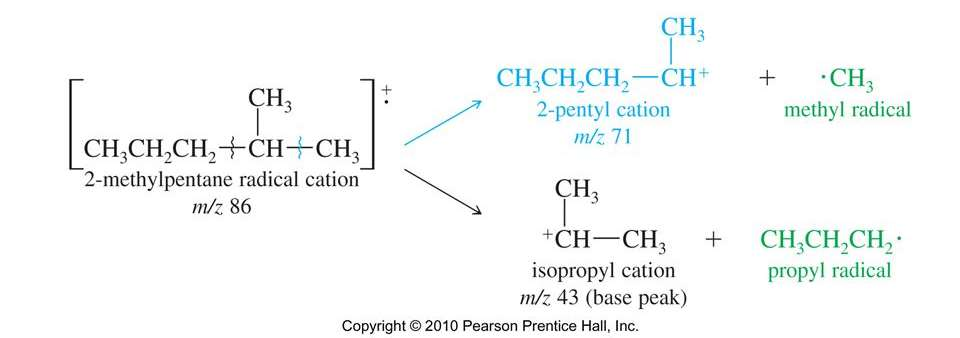
\includegraphics[width=0.9\textwidth]{2_039}
\end{figure}

Quindi per il 2-metilpentano, la frammentazione dello ione molecolare
($\nicefrac{m}{z}$ = 86) è possibile frammentare i due legami in \alpha{} alla
ramificazione. Il primo frammento ha $\nicefrac{m}{z}$ = 71, mentre il secondo
frammento ha $\nicefrac{m}{z}$ = 43.

\begin{figure}[H]
  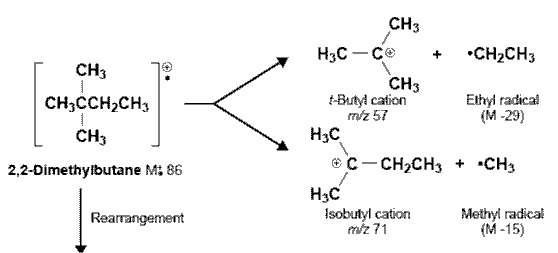
\includegraphics[width=0.9\textwidth]{2_038}
\end{figure}

Nel caso del 2,2-dimetilbutano, la frammentazione in \alpha{} può
avvenire in due legami differenti. Si possono quindi formare due
frammenti diversi, ovvero il catione isobutilico ($\nicefrac{m}{z}$ = 71) e il catione
t-butilico ($\nicefrac{m}{z}$ = 57). Questo spiega le differenze di abbondanza nel
profilo di massa.

\subsubsection{Alcani ciclici}

Nel caso degli alcani ciclici, si trova che lo ione molecolare è più
intenso rispetto a quello degli alcani, come si vede nello spettro del
cicloesano. Il picco molecolare è più intenso perché la molecola è più
difficile da frammentare, in quanto si devono rompere due legami.

La ionizzazione della molecola porta alla formazione di un catione
molecolare, che può essere delocalizzato.

\begin{figure}[H]
  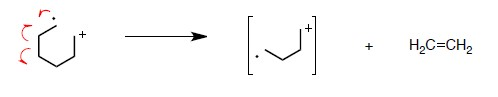
\includegraphics[width=\textwidth]{2_040}
\end{figure}

\fullpicture*{2_041}{Spettro del cicloesano}

La molecola non è stata rotta; per romperla, è necessario fare una
seconda rottura omolitica, che porta alla formazione di un secondo
catione radicale e di una molecola neutra.

Il radicale darà luogo ad un picco nello spettro di massa che sarà pari,
in quanto deriva dalla perdita di una molecola neutra.

Per un cicloesano con una catena carboniosa attaccata, come
l'etilcicloesano, si vedono, oltre alle frammentazioni tipiche
dell'anello, anche le frammentazioni tipiche della catena carboniosa.

\fullpicture*{2_042}{Spettro del etilcicloesano}

Nello spettro di massa, quindi, si trova lo ione molecolare ($\nicefrac{m}{z}$ = 112),
il picco base è a 83, che deriva dalla frammentazione in \alpha{} alla
ramificazione.

\subsection{Alcheni}

Per gli alcheni, lo ione molecolare è generalmente ben visibile. Però
gli alcheni presentano un problema, in quanto il doppio legame tende a
migrare nello ione molecolare e questo fa sì che sia impossibile
utilizzare la spettrometria di massa per capire dove si trova il doppio
legame nella struttura.

Ad esempio, prendendo come esempi gli spettri del 2-ottene e del
4-ottene, si vede che gli spettri sono praticamente identici.

È meglio non utilizzare mai la spettrometria di massa per localizzare un
doppio legame. Si può predire la frammentazione di un alchene, in quanto
si può prevedere che sarà favorita la frammentazione di un legame a-b,
rispetto all'instaurazione per dare un catione allilico e sono anche
possibili dei riarrangiamenti come diels-alder e mclafferty.

\fullpicture*{2_043}{Spettro dell'1-pentene}

\subsection{Alchini}

Lo ione molecolare è generalmente ben visibile. La spettrometria di
massa è particolarmente utile per identificare gli alchini terminali,
che danno due picchi in coppia nello spettro. Un picco si trova a M-1
(perdita di idrogeno) e il secondo picco a $\nicefrac{m}{z}$ = 39, che deriva dalla
frammentazione del legame \alpha-\beta{} rispetto al triplo legame, per
dare un catione propargilico.

\fullpicture*{2_044}{Spettro dell'1-pentino}

Ad esempio, lo spettro dell'1-pentino presenta uno ione molecolare, con
$\nicefrac{m}{z}$ = 68; si vedono i picchi diagnostici a M-1 (67) e a $\nicefrac{m}{z}$ = 39.

\subsection{Aromatici}

Per i composti aromatici, lo ione molecolare è molto intenso. Nei
composti aromatici, la spettrometria di massa è molto utile in quanto
sono presenti dei picchi diagnostici molto chiari.

Per gli alchilbenzeni, si trova sempre lo ione tropilio a $\nicefrac{m}{z}$ = 91,
inoltre si vede un cluster di picchi a $\nicefrac{m}{z}$ = 77, 78, 79. In ultimo si
possono trovare dei picchi abbondanti derivanti dalle frammentazioni con
perdita di acetilene M-26.

\pagebreak

Ad esempio, nello spettro dell'etilbenzene, si vede che lo ione
molecolare ha massa 106 ed è intenso. Il picco base è dato dal segnale
dello ione tropilio, con $\nicefrac{m}{z}$ = 91. Si vede anche il cluster di picchi a
77, 78 e 79, che sono poco intensi, ma sono comunque diagnostici per la
presenza di aromatici. Si vedono anche due picchi, a 65 e 39, che corrispondono alla
frammentazione secondaria, con perdita di acetilene, secondo la reazione

\begin{figure}[H]
  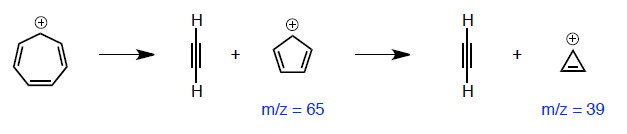
\includegraphics[width=0.8\textwidth]{2_046}
\end{figure}

\fullpicture*{2_045}{Spettro dell'etilbenzene}

\subsection{Alcoli}

Negli alcoli, lo ione molecolare è molto debole o assente. Sono presenti
dei picchi diagnostici; la frammentazione favorita è la rottura del
legame \alpha-\beta{} rispetto al gruppo funzionale. I picchi
diagnostici sono a $\nicefrac{m}{z}$ = 31, per alcoli primari, a $\nicefrac{m}{z}$ = 45, 59, 73,
\ldots{} (45 + 14n) per gli alcoli secondari e infine, per gli alcoli
terziari, si guardano i picchi a $\nicefrac{m}{z}$ = 59, 73, 81, \ldots{} (59 + 14n).

Altre perdite caratteristiche degli alcoli sono, la perdita d'acqua
(M-18) e la perdita di un idrogeno (M-1), o più (M-2).

Possono anche avvenire delle perdite con un meccanismo di tipo
McLafferty. I fenoli sono un po' particolari e possono dare anche
perdita di \ce{CO}.

\vfill

\pagebreak

\fullpicture*{2_047}{Spettro dell'1-pentanolo}

Ad esempio, lo spettro del 1-pentanolo, si vede che lo ione molecolare
ha massa pari (non sono presenti atomi di azoto), ed è poco intenso. Si
vede che questo spettro presenta i picchi caratteristici di un alcol
primario, come la perdita di acqua a M-18.

Si vede anche che è presente un picco a 31, che corrisponde alla
frammentazione del legame \alpha-\beta{}. Si vede inoltre la perdita di
due molecole neutre, per il picco a 42 (frammentazione secondaria) e si
vede anche il picco a M-43, che non è altro che la frammentazione della
catena alchilica.

\subsection{Ammine}

Le ammine sono molto simili agli alcoli; è favorita la rottura del
legame \alpha-\beta{} rispetto al gruppo funzionale. In ammine primarie
non ramificate, questa rottura comporta la formazione di un composto con
un picco diagnostico a $\nicefrac{m}{z}$ = 30.

\fullpicture*{2_048}{Spettro dell'esilammina}

Ad esempio, nello spettro di massa dell'esilammina, si vede che il picco
dello ione molecolare è molto debole; il picco base è a $\nicefrac{m}{z}$ = 30, che
corrisponde alla frammentazione in \alpha-\beta{}.

\fullpicture*{2_049}{Spettro di un ammina secondaria}

Per un ammina secondaria, lo ione molecolare ha un segnale debole; le
frammentazioni principali sono quelle dovute alla rottura del legame
\alpha-\beta{}. In questo caso sono possibili due rotture del legame
\alpha-\beta{} che danno luogo a due picchi, uno a 72 e uno a 58.

\vfill

\pagebreak

\subsection{Nitrocomposti}

I nitrocomposti si identificano molto facilmente dallo spettro di massa,
poiché la presenza di un gruppo nitro è diagnosticata dai picchi a M-46
(perdita di \ce{NO2}) e a M-30 (perdita di \ce{NO}). Il picco molecolare
è debole o assente, per un nitro alcano, ma è abbondante per un nitro
arene.

A volte si osservano anche gli ioni \ce{NO2+} e \ce{NO+}, con $\nicefrac{m}{z}$
rispettivamente uguale a 30 e 46.

\fullpicture*{2_050}{Spettro del nitrobenzene}

Ad esempio, guardando lo spettro del nitrobenzene, si vede che lo ione
molecolare è dispari, in quanto nella formula molecolare è presente un
atomo di azoto. Si vedono le due frammentazioni diagnostiche, con la
formazione dei picchi a 93 (perdita di \ce{NO}) e 77 (perdita di
\ce{NO2}). In entrambi i casi si è persa una molecola neutra, quindi i
picchi sono entrambi hanno una massa dispari

\subsection{Composti alogenati}

Nel caso particolare del cloro e del bromo, la spettrometria di massa
permette di diagnosticare la presenza di questi atomi partendo dai
picchi isotopici, in quanto presentano un picco isotopico a M+2 intenso.

Le frammentazioni principali sono:
\begin{itemize}
  \item perdita di alogeno
  \item perdita di acido alogenidrico \ce{HX}
  \item frammentazione del legame \alpha-\beta{}
\end{itemize}

\begin{figure}[H]
  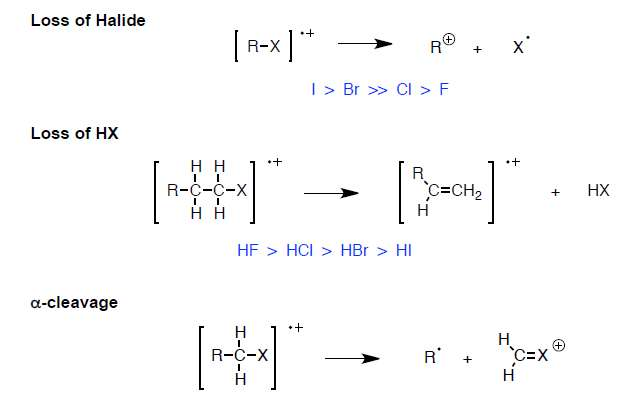
\includegraphics[width=0.8\textwidth]{2_053}
\end{figure}

Ad esempio, nello spettro del 1-cloropropano, si vede che lo ione
molecolare ha $\nicefrac{m}{z}$ = 78 e si vede anche il picco isotopico a M+2.
Misurando l'intensità dei due picchi, si vede che hanno un intensità di
3:1, quindi si ha un atomo di cloro.

La frammentazione del legame \alpha-\beta{} porta alla formazione del
catione con $\nicefrac{m}{z}$ = 49 (e anche 51 per via dei picchi isotopici). Il picco
base invece corrisponde ad un frammento con perdita di cloro, che ha
massa 43.

Si vede anche anche la perdita di \ce{HCl}, con $\nicefrac{m}{z}$ = 42, che è pari
perché deriva dalla perdita di una molecola neutra.

\begin{figure}[H]
  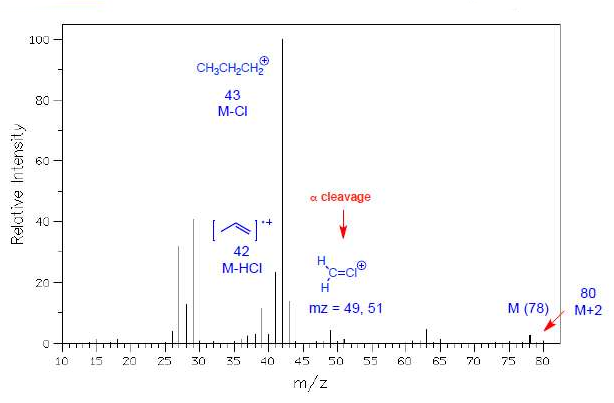
\includegraphics[width=\textwidth]{2_051}
  \caption{Spettro del 1-cloropropano}
\end{figure}

\vfill
\pagebreak

\subsection{Composti carbonilici}

I composti carbonilici hanno tre frammentazioni caratteristiche:
\begin{itemize}
  \item Frammentazione del legame in \alpha{} al carbonile. 
  Si possono rompere entrambi i legami; si formano due radicali ossonio.
  \item Si può anche rompere il legame in \beta.
  In questo caso, rompendo il legame in \beta,
  la carica positiva resta sul residuo R, mentre il radicale resta
  sull'ossigeno
  \item l'ultima frammentazione è il riarrangiamento di
  McLafferty, se sono presenti idrogeni in posizione \gamma.
\end{itemize}

\begin{figure}[H]
  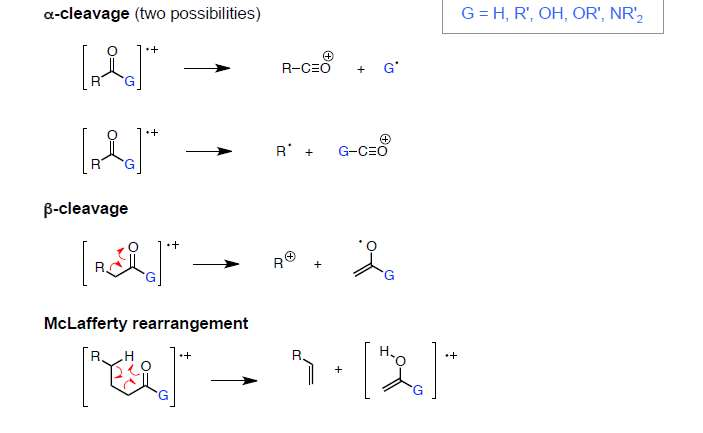
\includegraphics[width=0.9\textwidth]{2_052}
\end{figure}

Prendendo come esempio lo spettro del n-pentanale, si vede che lo ione
molecolare ha massa 86. La frammentazione può essere in \alpha, quindi
con perdita di idrogeno (85), oppure si può frammentare lungo la catena
carboniosa, quindi si ottiene un frammento con $\nicefrac{m}{z}$ = 29.

Questo composto può anche dare la frammentazione in \beta, quindi si
ottiene un catione formato da tre atomi di carbonio, con carica positiva
e $\nicefrac{m}{z}$ = 43.

Avendo anche degli idrogeni in posizione \gamma, è possibile anche avere
il riarrangiamento di McLafferty, che darà il catione radicale con $\nicefrac{m}{z}$ =
44.

\fullpicture*{2_054}{Spettro del n-pentanale}

L'ultimo esempio è lo spettro dell'acido butirrico. Nello spettro di
massa si vede che lo ione molecolare ha massa 88. La frammentazione in
\alpha porta ad uno ione M-17 o ad un secondo ione con $\nicefrac{m}{z}$ = 45.

È possibile anche il riarrangiamento di McLafferty, che fornisce un
catione radicalico con $\nicefrac{m}{z}$ = 60, che fornisce il picco base.

\fullpicture*{2_055}{Spettro dell'acido butirrico}

\vfill
\pagebreak


Di seguito sono presenti delle frammentazioni comuni per l'acido
butirrico

\begin{figure}[H]
  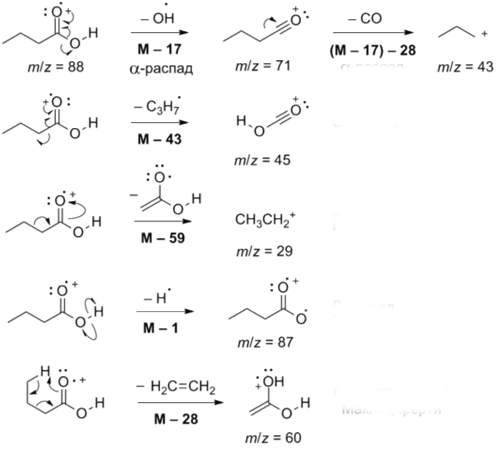
\includegraphics[width=0.8\textwidth]{2_056}
\end{figure}

La prima reazione riguarda la frammentazione in \alpha{} con M-17. La
seconda reazione è sempre una frammentazione in \alpha, che dà un
frammento a M-43. Si può anche avere una frammentazione in \beta. In
questo caso sono possibili due reazioni: la prima con M-59, mentre la
seconda con M-1. È anche possibile il riarrangiamento di McLafferty, che
comporta la formazione di uno ione con M-28.
